%%%%%%%%%%%%%%%%%%%%%%%%%%%%%%%%%%%%%%%%%%%%%%%%%%%%%%%%%%%%%%%%%%%%%
%
%  This is a sample LaTeX input file for your contribution to 
%  the MC2013 conference. Modified by R.C. Martineau at INL from A. 
%  Sood at LANL, from J. Wagner ORNL who obtained the original class 
%  file by Jim Warsa, LANL, 16 July 2002}
%
%  Please use it as a template for your full paper 
%    Accompanying/related file(s) include: 
%       1. Document class/format file: mc2013.cls
%       2. Sample Postscript Figure:   figure.eps
%       3. A PDF file showing the desired appearance: template.pdf 
%    Direct questions about these files to: richard.martinea@inl.gov
%
%    Notes: 
%      (1) You can use the "dvips" utility to convert .dvi 
%          files to PostScript.  Then, use either Acrobat 
%          Distiller or "ps2pdf" to convert to PDF format. 
%      (2) Different versions of LaTeX have been observed to 
%          shift the page down, causing improper margins.
%          If this occurs, adjust the "topmargin" value in the
%          mc2013.cls file to achieve the proper margins. 
%
%%%%%%%%%%%%%%%%%%%%%%%%%%%%%%%%%%%%%%%%%%%%%%%%%%%%%%%%%%%%%%%%%%%%%


%%%%%%%%%%%%%%%%%%%%%%%%%%%%%%%%%%%%%%%%%%%%%%%%%%%%%%%%%%%%%%%%%%%%%
\documentclass{mc2013}
%
%  various packages that you may wish to activate for usage 
\usepackage{graphicx}
\usepackage{tabls}
\usepackage{afterpage}
\usepackage{cites}
\usepackage{color}
\usepackage{amsmath,amsthm,amssymb}
\usepackage{verbatim}
\usepackage[parfill]{parskip}
\usepackage{tikz}
 
\newcommand{\N}{\mathbb{N}}
\newcommand{\Z}{\mathbb{Z}}
\newcommand{\deriv}[2]{\frac{\mathrm{d} #1}{\mathrm{d} #2}}
\newcommand{\pderiv}[2]{\frac{\partial #1}{\partial #2}}
\newcommand{\bx}{\mathbf{X}}
\newcommand{\ba}{\mathbf{A}}
\newcommand{\by}{\mathbf{Y}}
\newcommand{\bj}{\mathbf{J}}
\newcommand{\bs}{\mathbf{s}}
\newcommand{\B}[1]{\ensuremath{\mathbf{#1}}}
\newcommand{\Dt}{\Delta t}
\renewcommand{\d}{\mathrm{d}}
\newcommand{\mom}[1]{\langle #1 \rangle}
\newcommand{\xl}{{x_{i-1/2}}}
\newcommand{\xr}{{x_{i+1/2}}}
\newcommand{\il}{{i-1/2}}
\newcommand{\ir}{{i+1/2}}

\graphicspath{{figures/}}
 
%\usepackage{epsf}
%
%
% Insert authors' names and short version of title in lines below
%
\newcommand{\authorHead}      % Author's names here
   {S.R. Bolding and J.E. Morel}  
\newcommand{\shortTitle}      % Short title here
   {A HOLO method with ECMC for Thermal Radiative Transfer}  
%%%%%%%%%%%%%%%%%%%%%%%%%%%%%%%%%%%%%%%%%%%%%%%%%%%%%%%%%%%%%%%%%%%%%
%
%   BEGIN DOCUMENT
%
%%%%%%%%%%%%%%%%%%%%%%%%%%%%%%%%%%%%%%%%%%%%%%%%%%%%%%%%%%%%%%%%%%%%%
\begin{document}

%
%      Headers and Footers
\afterpage{%
\fancyhf{}%
\fancyhead[CE]{              
{\scriptsize \authorHead}}                                                
\fancyhead[CO]{               
{\scriptsize \shortTitle}}                  
%\lfoot{\scriptsize{
%International Conference on Mathematics and Computational Methods
%Applied to Nuclear Science \& Engineering (M\&C 2013), 
%\\ Sun Valley, Idaho, USA, May 5-9, 2013.}}%
\rfoot{\thepage/\totalpages{}}%

\pagestyle{fancy}
%\setlength{\topmargin}{-20pt}
}
 
\normalsize

\setlength{\baselineskip}{16.8pt}
\vspace{-3pt}

% 
% TITLE
%

\begin{center}
\textbf{\large \\%
A HIGH-ORDER LOW-ORDER ALGORITHM WITH EXPONENTIALLY-CONVERGENT MONTE CARLO FOR
THERMAL RADIATIVE TRANSFER\\
}
% 
% FIRST AUTHORS 
%
\setlength{\baselineskip}{14pt}
\textbf{S.R. Bolding and J.E. Morel} \\
Department of Nuclear Engineering\\
Texas A\&M University  \\
College Station, TX 77843 \\
sbolding@tamu.edu; morel@tamu.edu \\

% 
% SECOND AUTHORS (if not needed delete from here) 
%
\vspace{12pt}
\textbf{Double space and list Author C}\\
Department of Nuclear Engineering  \\
Name of University \\
Address \\
C@name.univ.edu\\ 
%
% SECOND AUTHORS (to here)
%

\end{center}

%
% SET RAGGED RIGHT MARGIN
%
\raggedright


\section*{ABSTRACT} 
\begin{quote}
\begin{small}
We have demonstrated the potential of a new high-order low-order (HOLO) algorithm for solving
thermal radiative transfer problems.  The low-order (LO) solver is based on spatial
and angular moments of the transport equation and a linear discontinuous
finite-element spatial representation.  
The LO solver is fully implicit in time and resolves the non-linear
temperature dependence at each time step.  The solution to the LO solver produces a
fixed-source, pure absorber transport problem as the high-order (HO) system.  The HO solver
utilizes exponentially-convergent Monte Carlo (ECMC) to give a globally accurate solution
for the angular intensity.  This global solution is used to compute consistency terms
that require the HO and LO solutions to converge to the same solution.  The use of ECMC
eliminates instabilities caused by statistical noise introduced to the LO consistency
terms.  Herein, we discuss the method in detail and compare initial results with an
implicit Monte Carlo code for one-dimensional gray test problems, as well as
demonstrate the efficiency of ECMC over SMC in this algorithm.

\emph{Key Words}: List of at most five key words

\end{small} 
\end{quote}

\setlength{\baselineskip}{14pt}
\normalsize

\Section{INTRODUCTION}

Thermal radiative transfer (TRT) physics are relevant in many high-temperature physical applications,
e.g., inertial confinement fusion and supernovae.  Such problems feature a strong
coupling between between the material and radiation energy balance equations, as well
as non-linear material and source term temperature dependences.  TRT problems often require solutions in a mix of
streaming and diffusive regions of the problem due to absorption-reemission physics
and opacity temperature dependencies. The diffusive regions are time
consuming to solve with higher-rank transport solutions and can be accurately
represented by a diffusion solution.  However, streaming regions require the accuracy of
a full transport treatment. 

Moment-based hybrid Monte Carlo (MC) methods have been proven useful for solving
non-linear, TRT problems. Recent work has focused on picard iteration high-order low-order
(HOLO) approaches~\cite{willert,park,rmc}.   Such methods utilize a low-order (LO) operator based on angular moments of the
transport equation, formulated over a coarse spatial mesh.
Physics operators that are time
consuming for the HO transport solver to resolve, e.g., the re-emission source and
physical scattering, are moved to the LO system.  
Newton methods allow for non-linearities in the LO equations to
be efficiently solved~\cite{willert}. This allows for non-linear
terms at each time step to be accurately resolved, eleminating the need for
approximate linearizations and short time steps relevant to other methods.

High-fidelity solutions can be achieved with HOLO methods by using standard
MC simulations to solve the HO transport
equation. The HO solution is used to construct consistency
terms that require the LO solution to be consistent with the HO solution.  These
consistency terms preserve
the accuracy of the MC solution method in the LO operator. Such HOLO algorithms suffer from stability issues caused by statistical noise introduced into the
consistency terms that are estimated via MC simulation.  
In this work, we demonstrate the utility of a unique LO operator in conjunction with
an exponentially-convergent Monte
Carlo (ECMC) method\cite{jake} for the HO solver.  The ECMC algorithm
allows for statistical noise to be reduced to the same order as the HOLO iteration
error with significantly less particles than standard MC. We have derived the LO operator
directly from the transport equation, using a linear-discontinuous (LD)
finite-element (FE) spatial
discretization, such that the
HO and LO solutions are consistent upon convergence. The LD spatial representation
mitigates issues with energy propagating faster than the speed of light by providing an
accurate spatial representation of the Planckian emission term within a cell.  We
present results for various Marshak wave test problems and reference are results
against IMC.

\Section{High-Order Low-Order Algorithm for Thermal Radiative Transfer}

\Subsection{Governing Equations} 

We have implemented a high-order low-order (HOLO) algorithm for the case of gray, one spatial dimension
TRT problems. For simplicity, we will also consider constant density and specific
heats throughout.  The governing equations are the radiation and
material energy balance equations, i.e.,
\begin{align}
    \frac{1}{c}\pderiv{I}{t} + \mu \pderiv{I}{x} + \sigma_t I
&= \frac{\sigma_s}{2} \phi +\frac{1}{2} \sigma_a a c T^4
  \\
  \rho c_v \pderiv{T}{t} &= \int_{-1}^{1} \sigma_a I^{n+1}(x,\mu)
\d\mu - \sigma_a a c (T^4),
\end{align}
where $\phi(x) = \int_{-1}^1 I(x,\mu) \d \mu$ is the scalar radiation intensity,
related to the energy density $E(x)=\phi(x)/c$. Here, $x$ is the position,  $\mu$ is
the $x$-direction cosine, and $a$, $c$, $\rho$, $c_v$, $\sigma_a$, $\sigma_s$, and
$\sigma_t$ are the radiation constant, speed of light, mass density, specific heat, absorption, scattering, and total
opacities (cm$^{-1}$), respectively.  The desired fundamental unknowns are the material
temperature $T(x)$ and radiation intensity $I(x,\mu)$.  In general, the material
properties are a function of $T$.
The equations are coupled through the gray Planckian emission source
$\sigma_a a c T^4$ and absorption term $\sigma_a \phi$.  
The notation of the scalar intensity $\phi$ is used throughout rather than the
typical radiation energy density $E=\phi(x)/c$.

MC solution to the TRT equations is typically achieved by the well-known
implicit Monte Carlo (IMC) method, first introduced by Fleck and Cummings~\cite{fnc}. This
method linearizes the emission source in the time derivative of the material energy
equation to eliminate the material energy equation from the system.  The remaining
transport equation is solved by MC with an effective scattering cross section representing
emission and reemission over the time step.  The time derivative in the transport
equation is solved continuously.  This
solution method is computationally expensive in diffusive regions of the problem due
to the high effective scattering, and is limited in time step size. 

A HOLO approach is a desirable alternative because
the LO method can easily resolve the solution in these diffusive regions.
For simplicity, our HOLO method will use a backwards Euler discretization in time, as
well as constant heat capacity and cell-wise constant opacity. The time discretized
equations are
\begin{align}
\mu \pderiv{I^{n+1}}{x} + \left(\sigma_t + \frac{1}{c \Delta t }\right) I^{n+1}
&= \frac{\sigma_s}{2} \phi^{n+1} +\frac{1}{2} \left(\sigma_a a c T^4
\right)^{n+1} + \frac{I^n}{\Delta t c} \label{ho_trans} \\
\rho c_v \frac{T^{n+1} - T^n}{\Delta t} &= \int_{-1}^{1} \sigma_a I^{n+1}(x,\mu)
\d\mu - \sigma_a a c (T^4)^{n+1} \label{lo_mat}.
\end{align}
where $\Delta t$ is the time step size and the superscript $n$ is used to indicate
the $n$-th time step.  The HOLO method will use moments of the above two equations to
resolve the non-linear temperature dependence between the two equations.  ECMC will
be used to solve the fixed source version of Eq.~\eqref{ho_trans} to provide
consistency terms in the LO system to correctly solve the problem.

\Subsection{Overview of the HOLO Algorithm}

In the HOLO context, the LO solver handles the physical scattering and
resolves the material energy spatial distribution.  The LO equations are based on
angular integrals and spatial moments formed over a finite element mesh of
Eq.~\eqref{lo_mat} and Eq.~\eqref{ho_trans}. The LO equations for the radiation
energy balance are similar to
double-$P_0$ equations, but with
spatially varying consistency parameters that are analogous to a variable
Eddington factor.  These consistency parameters are lagged in each LO solve,
estimated from the previous HO solve.  
If the angular consistency parameters were estimated exactly, then the LO equations are exact with respect to the chosen
spatial discretization. The material energy equation consists of only spatial moments and does not contain
any consistency terms, providing energy conservation. The HO solver is not required
to conserve energy.

The solution to the LO system is used to construct a spatially LD representation of
the scattering and emission sources on the right hand side of Eq.~\eqref{ho_trans}.  This defines a fixed-source, pure absorber
transport problem for the HO operator.  This transport problem, which we refer to as the HO problem, is solved using ECMC with adaptive mesh
refinement.  The HO problem defines a characteristic method that uses MC to
invert the continuous streaming plus removal operator with an LD representation of
the source terms (including inscattering).  The ECMC algorithm allows for the statistical noise in the MC
solution to be efficiently reduced to any desired precision within the limits of computational memory.  Thus, the HO solve produces a
globally-accurate, LD representation of the angular intensity
$\tilde{I}(x,\mu)$.  Here, we emphasize that the ECMC algorithm computes a
projection of the exact solution onto a LDFE space-angle trial space, rather than a
standard FE solution.  This is in general far
more accurate than a standard FE solution. 

Once computed, the projected LD
angular intensity $\tilde{I}(x,\mu)$ is used to evaluate the LO
consistency parameters for the next LO solve.  Since there is a global, functional representation of
the angular intensity,  LO parameters are estimated using quadrature and do not require additional tallies.  The HO solver does not
produce a new temperature in the thermal radiative transport (TRT) context; it is
only used to estimate the angular parameters in the LO solution, which eliminates
typical operator splitting stability issues that require linearization of the emission source.

The process of a LO estimate of the transport sources for the HO solver, followed by
an ECMC
solve to estimate LO parameters, represents one HOLO fixed-point iteration.
The consistency terms force the HO
and LO solutions for $\phi(x)$ to be consistent to the order of the current HOLO
iteration error.  The solution for $T(x)$ is only estimated via the LO solution
(which preserves the accuracy of the HO solution). 
The HOLO iterations are performed until the solutions are converged to a
desired precision, within each time step.  Currently, the HOLO convergence criteria is based on
the convergence of the FE representation of $\phi^{n+1}(x)$ between successive HOLO iterations
$k$. The HOLO algorithm, for each time step, is

\begin{enumerate}
    \item Perform a diffusion-equivalent solve of the LO system to produce $T^0(x)$
        and $\phi^(0)(x)$ at $t_{n+1}$
\item Solve the HO system for $\tilde{I}^{k+1/2}(x,\mu)$ using ECMC, based on the current
    LO estimate of the right hand emissiion and scattering sources.%$\sigma_s(T^k)\phi^{k}$ and $B(T)^{k}$.
\item Compute LO consistency parameters with $\tilde{I}^{k+1/2}$.  
\item Solve the LO system using new HO consistency parameters to produce a new
    estimate of $\phi^{k+1}$
    and $T^{k+1}$ at $t_{n+1}$.
\item Repeat 2 -- 4 until convergence is achieved.
\item Move to the next time step.
\end{enumerate}


\Section{The Low-Order Solver for the Radiative Transfer Equations}

The LO system is formed by taking spatial basis moments and half-range angular
integrals of Eq.~\eqref{ho_trans} and Eq.~\eqref{lo_mat}. The spatial moments are taken over each spatial cell $i$:
$x\in[x_{i-1/2},x_{i+1/2}]$, weighted with the standard linear Lagrange
interpolatory basis functions.  For example, the $L$  moment operator is defined by
\begin{equation}\label{x_mom}
\mom{\cdot}_{L,i} = \frac{2}{h_i} \int_{x_{i-1/2}}^{\xr} b_L(x) (\cdot) \d x,
\end{equation}
where $h_i=x_{i+1/2}-x_{i-1/2}$ is the width of the spatial element and
$b_L(x)=(x_{i+1/2}-x)/h_i$ is the FE basis function corresponding to position
$x_{i-1/2}$.  The right moment $\mom{\cdot}_R$ is defined with weight function $b_R(x)=(x -
x_{i-1/2})/h_i$.  Here, it is emphasized that $\phi_{L,i}$ and $\phi_{R,i}$ represent
the values of the scalar intensity at $x_\il$ and $x_\ir$ that preserve the zeroth
and first moments over the cell, not to be confused with $\mom{\phi}_L$ and
$\mom{\phi}_R$, which
represent a volume-averaged moments.
The positive and negative half-range integrals of the angular flux are defined as
$ \phi^+(x) = \int_0^{1} I(x,\mu) \d \mu$ and $ \phi^-(x) = \int_{-1}^{0} I(x,\mu) \d
\mu$, respectively.  Thus, in terms of half-range quantities, $\phi(x) = \phi^-(x) + \phi ^+(x)$.  

Pairwise application of the $L$ and $R$ basis
moments with the $+$ and $-$ half-range integrals to Eq.~\eqref{ho_trans} equation
ultimately yields four radiation balance
equations, for each cell.  For example, the equation resultion from application of the $L$ moment and
positive half-range integral is
\begin{multline}\label{lo_tran}
    -2{\mu}_{i-1/2}^{n+1,+} \phi_{i-1/2}^{n+1,+} + \mom {\mu}_{L,i}^{n+1,+}
  \mom{\phi}_{L,i}^{n+1,+}
  +  \mom\mu_{R,i}^{n+1,+}
  \mom{\phi}_{R,i}^{n+1,+} +  \left(\sigma_t^{n+1}+\frac{1}{c \Delta t} \right) h_i 
  \mom{\phi}_{L,i}^{n+1,+} \\-  \frac{\sigma_s h_i}{2} \left( \mom{\phi}_{L,i}^{n+1,+} +
  \mom\phi_{L,i}^{n+1,-}\right) = \frac{h_i}{2} \mom{\sigma_a^{n+1} a c T^{n+1,4}}_{L,i} +
  \frac{h_i}{c\Delta t}\mom{\phi}_{L,i}^{n,+},
\end{multline}
where the $\mom{\phi^\pm}$ terms represent volumetric and angular averaged fluxes,
and the $\phi_{i-1/2}$ term represents an angular average over a face.  The moments
of the source term will be defined later on. The $-$ direction equations are
essentially the same with $+ \rightarrow -$ (there is also
a difference in the upwinding and extrapolated face terms, explained below). 
The angular consistency terms are defined in terms of half-range averages, e.g.,
\begin{equation}\label{const}
\mom{{\mu}}_{L,i}^+ =  \frac{
{\displaystyle \frac{2}{h_i}} \int\limits_0^1 \int\limits_\xl^\xr \mu \, b_L(x)
I^{n+1}(x,\mu) \d x \d \mu } 
{{\displaystyle \frac{2}{h_i}} \int\limits_0^1 \int\limits_\xl^\xr \, b_L(x)
I^{n+1}(x,\mu) \d x \d \mu } .
\end{equation}
The consistency terms for the $R$ basis moment and $\mu_{i\pm1/2}^\pm$ face
terms are defined analogously. 

To derive the LO material energy equations, first $T(x)$ is assumed to be in the LD trial space, i.e.,
$ T(x) \simeq T_{L,i} b_L(x) + T_{R,i} b_R(x),\quad x\in(x_{i-1/2},x_\ir)$.
Similarly, the emission term is represented in the material and radiation equations with the LDFE
interpolant $\sigma_{a,i}acT^4(x) = \sigma_{a,i}ac\left[T_{L,i}^4 b_{L}(x) +
T_{R,i}^4 b_R(x)\right]$.  
 The $L$ and $R$ spatial moments are taken of the material energy equation, using the
 LDFE
 definition for $T(x)$ and $T^4(x)$. For example, the final LO material energy
 equation resulting from application of the $L$ moment is
\begin{multline}
    \frac{\rho c_v}{\Delta t}\left[ \left(\frac{2}{3}T_{L,i} + \frac{1}{3}T_{R,i}
        \right)^{n+1} - \left(\frac{2}{3}T_{L,i} + \frac{1}{3}T_{R,i}
    \right)^{n} \right]  + \sigma_a^{n+1,k+1} \left( \mom{\phi}_{L,i}^+ +
    \mom{\phi}_{R,i}^- \right)^{n+1} \\ = \sigma_a^{n+1}a c
\left( \frac{2}{3} T_{L,i}^4 + \frac{1}{3}T_{R,i}^4
        \right)^{n+1}.
\end{multline}

\Subsection{Closing the Non-Linear System}

The six degrees of freedom (DOF) over each cell $i$ are the four moments $\mom{\phi}_{L,i}^+$,
$\mom{\phi}_{R,i}^+$, $\mom{\phi}_{L,i}^-$, and $\mom{\phi}_{R,i}^-$ and the two
spatial LDFE edge values $T_{L,i}$ and $T_{R,i}$. The four radiation and two material
energy equations define a system of equations for the six DOF without additional
discretization.  However, the consistency parameters (e.g., Eq.~\eqref{const}) are not known a priori, and
there is no relation between the volume and face averaged quantities. We will use the
HO solver to close these equations.  

A lagged estimate from the previous HO solve is
used to estimate the angular consistency parameters. In the HOLO
context, the equations for LO unknowns at iteration $k+1$ use consistency parameters
computed using Eq.~\eqref{const} with the latest HO solution $\tilde{I}^{n+1,k+1/2}$
as an approximation for $I^{n+1}$. For the initial LO
solve, all average $\mu$ parameters are
set to $\pm 1/\sqrt{3}$, yielding a solution equivalent to an S$_2$ solution.  For this initial S$_2$ solve, it is necessary
to renormalize radiation boundary conditions to get an accurate solution and preserve
conservation, which is standard in $S_N$ methods.
To close the LO system spatially, the usual LD upwinding
approximation is used.  For example, for Eq.~\eqref{lo_tran}, the face terms $\mu_{i-1/2}$ and $\phi_{i-1/2}$
terms are upwinded from the previous cell $i-1$ or from a boundary condition; the terms
at $x_{i+1/2}$ are linearly extrapolated, computed using the $L$ and $R$ basis moments.
Because the HO
solver uses an LD representation, this LO spatial closure is inherently
consistent.  Because there are no
spatial temperature derivatives, there is no evaluation of $T$ at faces and thus no need for an
upwinding closure.  

\Subsection{Alternative Closure Near the Wave Front}

The LD closure is not strictly positive.  In particular, for
optically thick cells with a highly varying temperature distribution, the solution is driven negative.  In thick regions of
TRT problems, reasonably fine spatial cells can still be on the order of millions of mean
free paths; negativities with LD are simply unavoidable in these cells and mesh
refinement is of minimal use.  Typically, for a standard LDFE method,
the equations are lumped to produce a strictly positive solution. However, standard FE lumping
procedures would make computing the consistency terms from the HO solver difficult. 
An alternative discontinuous spatial discretization is used that uses a relation between the
spatial moments and outflow that produces the same result as the
standard FE lumping procedure.  

The $L$ and $R$ moments are defined the same as before,
preserving the same average with in a cell, but the relation between the moments and
the outflow is modified to force a strictly positive outflow.   For example, for positive $\mu$,
the outflow is now defined as
\begin{equation}
    \phi^+_{i+1/2} = \mom{\phi}_R^+.
\end{equation}
This is different than the standard extrapolated outflow for LD given by $\phi^+_{i+1/2} = 2\mom{\phi}_R^+ - \mom{\phi}_L^+$. 
Because the basis function $b_R(x)$ is strictly positive, the above moment and thus outflow is
inherently positive.  This spatial discretization is second order, as compared to the 
third order of standard LD.  The same upwinding as before is used for this
discretization. This closure is only used in cells in which negativities occur.

\Subsection{Solving the Non-Linear LO system}

We have used Newton's method to solve the global system of coupled LO
equations, based on a typical linearization of the Planckian source with opacities
evaluated at lagged temperatures, as described in~\cite{morel_newton}.  Application of the first order Taylor expansion in time of the
gray emission source $B(T)$, about some temperature $T^*$ at some
time near $t^{n+1}$ gives
\begin{equation}\label{new_planck}
    \sigma_a^* a c T^{4,n+1} \simeq \sigma_a^* a c \left[T^{*4} + (T^{n+1} - T^*) 4T^{*3} \right]
\end{equation}
where the superscript $*$ denotes evaluation at $T^*$. This expression is substituted for the
emission term in the time discretized material
energy equation given by Eq.~\eqref{mat_eq}.  The resulting equation is manipulated
to provide an explicit expression for $T^{n+1}$ as a
function of $T^*$ and an effective scattering source
\begin{equation}
\label{lo_t_new}
T^{n+1}  = \frac{1}{\rho c_v } f\sigma_a^* \Delta t \left( \phi^{n+1} - c a T^{*4} \right)
+ f T^n + (1-f) T^*.
\end{equation}
where $f^* = (1 + \sigma_a^* c \Delta t \beta^*)^{-1}$ with
$\beta^* = \frac{4 a T^{*3}}{\rho c_v}$ and the superscript $^*$ indicates evaluation
at $T^*$. The
expression for $T^{n+1}$ can be substituted back into Eq.~\eqref{new_planck} to form
an explicit approximation for the emission source at $t_{n+1}$ as
\begin{equation}\label{t_next1}
    \sigma_a a c T^{4,n+1} \simeq \sigma_a^* (1 -f^*) \phi^{n+1}
    + f^* \sigma_a^* a c T^{4,n} + \rho c_v\frac{1-f^*}{\Delta t} (T^N - T^*)
\end{equation}

Based on a guess for $T^*$, the above equation gives an expression for
the Planckian emission source in the right hand side
of Eq.~\eqref{lo_tran} with an additional effective scattering source.
This allows for four linear equations for the four remaining radiation unknowns to be fully
defined.  The final equation for the left basis moment and positive flow, for constant
$f^*$ and $\sigma_a^*$ over a cell, becomes
\begin{multline}\label{lo_trans_fin}
    -2{\mu}_{i-1/2}^{n+1,+} \phi_{i-1/2}^{n+1,+} + \mom {\mu}_{L,i}^{n+1,+}
  \mom{\phi}_{L,i}^{n+1,+}
  +  \mom\mu_{R,i}^{n+1,+}
  \mom{\phi}_{R,i}^{n+1,+} +  \left(\sigma_t^*+\frac{1}{c \Delta t} \right) h_i 
  \mom{\phi}_{L,i}^{n+1,+} \\- \frac{h_i}{2}\left(\sigma_s^* + \sigma_a^*(1-f^*)\right)
  \left( \mom{\phi}_{L,i}^{n+1,+} +
  \mom\phi_{L,i}^{n+1,-}\right) = \\ \frac{1}{2} h_i \sigma_a^*a c f^* \left(\frac{2}{3} T_{L,i}^{4,n} +
  \frac{1}{3} T_{R,i}^{4,n} \right) + 
  \frac{h_i}{c\Delta t}\mom{\phi}_{L,i}^{n,+}
\end{multline}

Once these linear equations have been solved for $\phi^{n+1}$, a new estimate of
$T^{n+1}$ can be determined using Eq.~\eqref{lo_t_new}, providing energy
conservation.  To account for spatial dependence, Eq.~\eqref{lo_t_new} can simply be evaluated
at the edge values in a cell, e.g., with $\phi^{n+1}_L$ and $T^*_L$ to get $T_L^{n+1}$.

Based on these equations, the algorithm for solving the LO system is defined as
\begin{enumerate}
    \item Guess $T^*_L$ and $T^*_R$, typically using $T^n$.
    \item  Build the LO system based on the effective scattering $\sigma_a^*(1-f^*)$ and emission terms
        (i.e., evaluation of  Eq.~\eqref{lo_trans_fin}).
    \item Solve the linearized LO system to produce an estimate for $\phi^{n+1}$.
    \item Evaluate a new estimate of the $T_{L,i}$ and $T_{R,i}$ at the end of the time step
    $\tilde{T}^{n+1}$ using Eq.~\eqref{new_temp}.
    \item $T^*\leftarrow\tilde{T}^{n+1}$.
    \item Repeat 2-5 until $\tilde T^{n+1}$ and $\phi^{n+1}$ are converged.
\end{enumerate}

\Section{The ECMC High Order Solver}

The HO solver must solve a fixed source, pure absorber transport
problem.  We will solve this equation using ECMC. A more detailed description of the
ECMC method can be found in~\cite{jake_thesis}. In the
HOLO context, the sources are estimated by the previous LO solve.
The equation with HOLO iteration indices is
\begin{equation}
\mu \pderiv{I^{n+1,k+1/2}}{x} + \left(\sigma_t^k + \frac{1}{c \Delta t }\right)
I^{n+1,k+1/2}
= \frac{\sigma_s^k}{2} \phi^{n+1,k} +\frac{1}{2} \left(\sigma_a^k a c T^4
\right)^{n+1,k} + \frac{\tilde I^n}{c\Delta t} 
\end{equation}
where $k$ represents the outer HOLO iteration index.  Material property indices will be
suppressed from now on.  Here, $k+1/2$ denotes the
HO solve within HOLO iteration $k$, whereas $k$ and $k+1$ represent successive LO
solves.  In operator notation, the previous equation can be written as
\begin{equation}\label{te_oper}
\B L^k \psi^{k+1/2}  = q^{k}
\end{equation}
where $\psi^{k+1/2}$ is the solution of the angular intensity $I^{n+1}$ based on the $k$-th
estimate of $q^k$.
The linear operator $\B L^k$ is the streaming plus
removal operator defined by the left hand
side of Eq.~\eqref{ho_trans}, and $q^k$ is defined by the LD representation of the
right hand side, as estimated via the $k$-th LO solve.  

To define the ECMC algorithm, the HO-LO iteration indices
$k$ are dropped, as the LO estimated $q^{k}$ and $\B L^{k}$ remain constant over the entire HO solve.
The $i$-th approximate solution to Eq.~\eqref{te_oper} ($i$ represents inner HO
batches) is represented as
$\tilde{\psi}^{(i)}$.    
The $i$-th residual is 
\begin{equation}
r^{(i)} = q - \B L\tilde{\psi}^{(i)}.
\end{equation}
Addition of $\B L\psi - q=0$ to the above equation 
and manipulation of the result yields the error equation
\begin{equation}
    \B L (I^{n+1} - \tilde{\psi}^{(i)}) = \B L \tilde{\epsilon}^{(i)} = r^{(i)}
\end{equation}
where $I^{n+1}$ is the exact solution and $\tilde{\epsilon}^{(i)}$ is finite element
representation of the error in
$\tilde{\psi}^{(i)}$. The above equation is inverted yielding the Monte Carlo
estimate of the error in $\tilde{\psi}^{(i)}$, i.e.,
\begin{equation}
\tilde{\epsilon}^{(i)} = \B L^{-1} r^{(i)}
\end{equation}
where $\B L^{-1}$ is the Monte Carlo inversion of the streaming and removal operator.
The solution $\tilde{\psi}^{(i)}$ represents the projection of the exact Monte Carlo
solution onto the trial space, rather than a standard finite element solution.
For example, the LD trial space preserves the zeroth and first spatial moment over a
cell; the zeroth moment is computed using a standard path-length volumetric flux tally, which
is equivalent to typical volumetric averages computed in Monte Carlo calculations.  The primary truncation error is in the LD
representation of the right hand side source terms and residual at each
iteration.  The only tallies used are volumetric flux tallies over all of the finest space-angle
elements; tallies are computed for the average, slope in $x$, and slope in $\mu$ of
$I^{n+1}(x,\mu)$.  

The HO solver requires an LD representation of the Planckian emission sources.  For cell-wise constant cross section, the
representation takes the form $B(T,x) = \sigma_a a c (T_L^4 b_L(x) + T_R^4 b_R(x)$. 
For reference, for Eq.~\eqref{ho_trans} the residual at iteration $i$ in the HO solve
is
\begin{equation}
r^{(i),k+1/2} = \frac{\sigma_s}{2} \phi_{LD}^{n+1,k} +\frac{1}{2} \left(\sigma_a^* a T^4
\right)_{LD}^{n+1,k} + \frac{\tilde{I}^n}{\Delta t c} -
\left(\pderiv{\tilde{I}^{n+1,k+1/2}}{x} +
\left(\sigma_t + \frac{1}{c \Delta t }\right) \tilde{I}^{n+1,k+1/2}\right)^{(i)}
\end{equation}
where the $k$ terms are LD in space on the coarsest mesh and are not recalculated at any point during
the HO solve.  The functional form of $\tilde{I}^n$ is defined over the finest mesh from the last HOLO
iteration of the previous time step.  For simplicity, $\tilde I^n$ is projected onto the current mesh in the HO solve.
  
An initial guess for the angular intensity is computed based on the previous solution
for $I^{n}$, or for a later HOLO iteration from the last batch estimate from the previous
HO solve. This is an important step, and significantly reduces the required number of
particles per time step because $I$ does not change drastically between time steps in
highly diffusive problems.  The initializations are
computed as a projection of the solution onto the initial coarsest mesh.

  The ECMC algorithm is
\begin{enumerate}
    \item Initialize the guess for $\tilde{I}^{n+1,(0)}$ to $\tilde{I}^{n}$ or the
        projection of $\tilde{I}^{n+1}$ from the latest HO solve
\item Compute $r^{(i)}$.
\item Solve $\tilde{\epsilon}^{(i)} = \B L^{-1} r^{(i)}$
\item Compute a new estimate of the intensity $\tilde I^{n+1,(i+1)} = \tilde I^{n+1,(i)}
+ \tilde\epsilon^{(i)}$
\item Repeat steps 2 -- 4 until desired convergence criteria is achieved. 
\end{enumerate}

Currently, the convergence criteria is based on the $\|\tilde{\epsilon}^{(i)}\|_2$, i.e.,
\begin{equation}
\|\tilde{\epsilon}^{(i)}\|_2 = \int_\mathcal{D} \int_{-1}^1
\tilde{\epsilon}^{(i)}(x,\mu) \d\mu \d x\leq \text{TOL}.
\end{equation}
Exponential convergence is obtained because with each inversion of $\B L$ a
better estimate of the solution is being used to compute the new residual, decreasing
the magnitude of the Monte Carlo source each iteration $i$.  Each Monte Carlo
estimate for the error has a sample mean that contains a statistical distribution that decreases 
by the standard $1/{N}$ reduction in variance, however the 
angular intensity can obtain a higher convergence rate because of the new information about the
solution introduced each iteration.  If the statistical estimate of $\tilde\epsilon$ is not sufficiently
accurate, then the iterations would diverge.  Currently, the error is montitored and
ensured to not be too large, relative to $\epsilon$.

Because the exact angular intensity does not in general lie within the LD trial space, the
iterative estimate of the error will eventually stagnate once the error cannot be sufficiently
represented by a given LDFE mesh.  An adaptive $h-$refinement algorithm is used
to allow the system to continue converging towards the exact solution.  Once the
error has stagnated, refinement is performed on some percentage of the cells
based on the jump errors over each face of a space-angle cell.  Each space-angle cell
to be refined is divided into four equal-sized cells.  The previous estimate of the
angular intensity is projected onto the new cells.(resulting in a continuous solution over
each of the cells); this is an inaccurate solution over the new mesh, and thus the
first iteration after refinement will result in an increase in the error.  The error
is also increased due to the new, more accurate projection of $\tilde I^n$ onto the
new mesh.  However, typically within in one more iteration the error will have
decreased past the error prior to refinement.  

 It is also noted that the trial space
representation of the HO angular intensity contains most of the information necessary to
estimate the exact Monte Carlo projection of the LO parameters (the average and first moments of the angular intensity
in angle and space), except for the cross moment ($\langle x \mu \rangle$).  However,
because the LD angular intensity representation is accurate over the refined HO mesh, that
functional form can be used to estimate the cross moment on the LO mesh with a
similar degree of accuracy.  

\Subsection{Continuous Energy Deposition Tracking}

As in~\cite{cwd}, we will exponentially attenuate particles to reduce statistical
variance in the tallies.  Because the ECMC problem solves a pure-absorber problem,
particles can be allowed to stream, with their weight deterministically modified
along the path.  Because the particles are exponentially attenuated, the weight is
adjusted as $w(x) = w(x_0)exp(-|(x-x_0)/\mu|)$.  The tallies are modified to account
for this weight exponential attenuation by evaluating the integral along the path
length. 

\Subsection{Source Bias}

A modified stratified sampling method has been used to effectively distribute particle
histories throughout the problem. The residual gives a good indication of where
particles are most likely to contribute to the error, particularly in diffuse
problems.  In higher dimensions a more accurate weighting that accounts for the
proability of particles in one region contributing to particles in another region may
be necessary.  

In the modified sampling algorithm the number of particle histories sampled in
each cell is proportional to the magnitude of the residual in each cell, unless the
number of particles in a cell is below some minimum. In this case, a minimum number
of histories, specified by the user, is placed in cells below the minimum. This is to
prevent bad statistics in certain cells, particularly in the case of adaptively
refined meshes.  There is
also a relative probability cutoff such that cells with an insignificant
residual will have no histories sampled there. In these regions the problem is
remaining in steady state and the solution is known exactly.  The cutoff is set
relative to equal probability of being born in each cell and is adjusted to account
for the fact that smaller cells have lower probability.  By ensuring sampling of each
significant region of phase space, energy is locally conserved more accurately.   

%The unmodified probability of a particle being born in cell $j$ is 
%\begin{equation}
%p_j = \frac{||r^{(i)}_j||}{||r^{(i)}||}
%\end{equation}
%Thus, the number of
%particles in cell $j$ is 
%\begin{equation}
%N_j = 
%\left\{\begin{matrix}
% \lfloor(Np_j)\rfloor, & Np_j > N_{\min}
%\\ 0, & \frac{p_j}{1/N_c} < p_{cut}
%\\ N_{min}, & \text{else}
%\end{matrix}\right.
%\end{equation}
%where $N_{\min}$ is the minimum number of histories in significant cells, $N_c$  is the number of cells, and $p_{cut}$ is the chosen relative probability cutoff.
 The implementation of the above equation is modified such that the total number of histories is as
close to original requested number of histories as possible. This is done by first filling the cells with $N_{min}$ histories and distributing the remaining number of histories proportional to $p_j$.

\Subsection{Fixup Near the Wave-Front}

In cells near the wave front, the LD trial space results in negativities as with the
LO solver.  Currently, we just check the consistency terms at the end of the HO solve
and detect if they lie in the appropriate half-space.  If the terms are non-physical, then
they are set to diffusion-equivalent terms.  This may lead to artificially fast
wave-speeds in certain cells.  A better alternative would be to switch to another
trial space in these cells that is strictly positive.  


\Section{Results}

To demonstrate this method we will compare the results of our method with IMC with
source tilting, which should be effectively solving the same problem.  It is not easy
to compare the two results with out an analytical solution for a Marshak wave.  
These results are presented to verify that with sufficient particle histories
to converge the problem our code is getting accurate
solutions and to demonstrate issues to be resolved in future work.  Future
publications will focus on iteration counts and using a limited number of particles.
The radiation energy
distribution is plotted as an equivalent temperature given by
$T_r=\sqrt[4]{\phi/(ac)}$.  Although Thompson scattering
can be handled by the LO solver in this method, we have only considered pure absorber
problems here.  We have demonstrated this method with scattering included in the
Eigenvalue solves~\eqref{ans_2014}.

For all problems, a relatively high HOLO iteration relative error tolerance of 1.E-02 between
radiation energy distributions was used, leading to only one HO solve being performed
per time step to limit simulation times.  A tolerance of 1.E-06 was used for the LO
solver and 5.E-03 for the HO solver.  To ensure convergence of the HO solver, a
relatively large number of histories per batch $>150000$ was used,
unless otherwise noted.   This is a sufficiently
high number of histories that for the majority of time steps HO solver is converged within 2
batches; in reality more efficient error reduction could be achieved by using more
batches with less particles per batch.  It is important to note that because there is no scattering, each history can be solved more efficiently than in IMC.  Adaptive mesh refinement and more batches
were used as necessary (typically in optically thin regions) by the
solver, testing this aspect of the code.  All meshes begin with 200 spatial cells and
two angular cells in each half-range.

\Subsection{Constant Solution Infinite Medium}

To check the basic functionality of the HOLO algorithm a constant solution
representing an infinite medium was performed, with results shown in Fig~\ref{constant_fig}.  Even though the LO solver can get the
solution exactly right, we forced the residual to sample 2500 particles per time step.  Because of
the initial guess of $\tilde I^n$ for the radiation, the residual source is very small in
this case and the statistical noise is on the order of roundoff for the ECMC solver.
In general, regions that are in steady state will not sample residual particles.
  For the IMC results, statistical noise is relevant even for a constant solution for the
unless significantly more than 2500 particles per time step is used. 
\begin{figure}[htb]
   \centering
   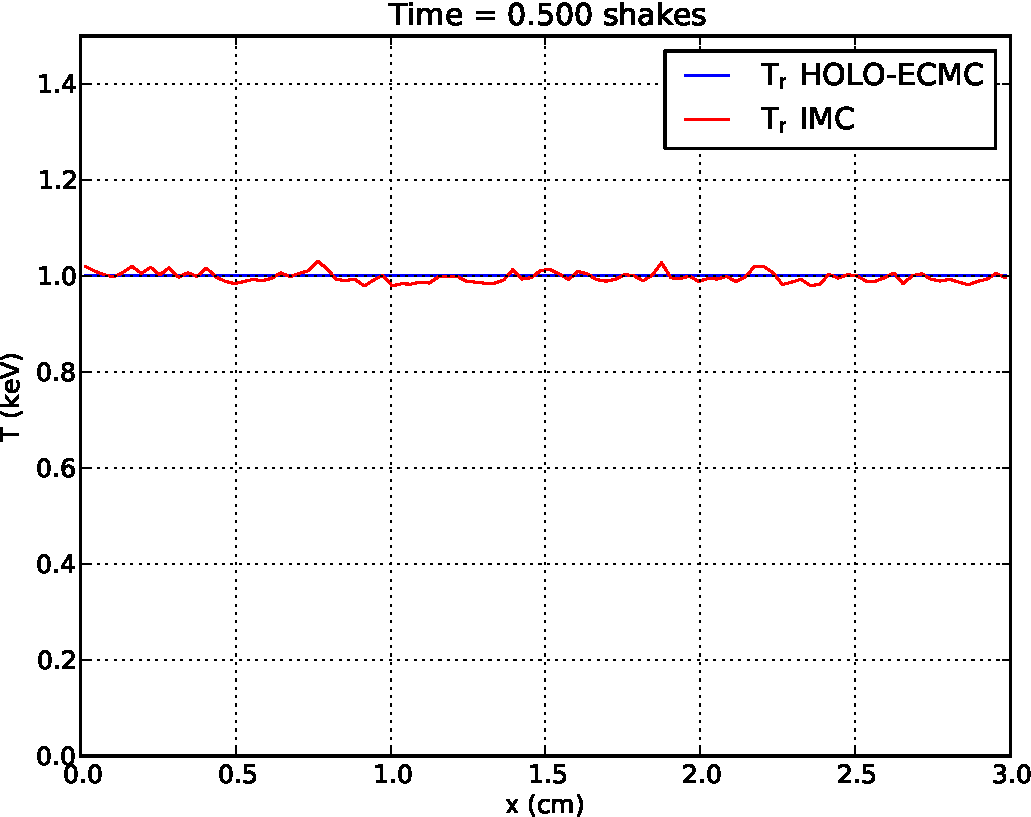
\includegraphics[width=0.6\textwidth]{constant.pdf}
   \caption{\label{constant_fig} Comparison of IMC and HOLO-ECMC results for
       an equilibrium solution.}
\end{figure}


\Subsection{Two Material Problem}

This problem consists of an optically thin and an optically thick material region,
with constant cross sections.  This problem demonstrates the utility of the
hybrid method in both the streaming (left) and diffuse (right) regions of the domain.  The material properties are given in
Table~\ref{two_mat_props}.  Initially the radiation and material energies are in
equilibrium at a temperature of 0.05 keV.  An isotropic incident intensity of 0.500 keV
is applied at $x=0$ at $t=0$; the incident intensity on the right boundary is 0.05
keV.  The simulation was ran for 5 shakes with a
time step size of 0.001 shakes.  

Fig.~\ref{twomat_quick} compares the HOLO, IMC, and diffusion computed radiation temperatures at $t=0.010$ sh.  Both curves plot the cell-wise averages rather than the LD representation.  At this point in the simulation, the radiation is in the optically thin region of the problem, so the diffusion solution has propagated too quickly.  The IMC and HOLO methods agree well.  Fig~\ref{twomat_full} compares the IMC and HOLO radiation temperature profiles at the end of the simulation.  The wave fronts show good agreement.  
These results were computed using the lumping-equivalent discretization for the LO solver, noting that this is not consistent with the HO solver.  A consistent discretization in the HO solver would likely produce a more accurate solution. 
\begin{table}[htb]
    \begin{center}
        \begin{tabular}{|c|cc|}  \cline{2-3}
            \multicolumn{1}{c|}{}   & $x \in [0,0.5)$ cm & $x \in [0.5,1.0]$ cm   \\ \hline
            $\sigma_a$ (cm$^-1$)  & 0.2 & 2000 \\
            $\rho$ (g cm$^-3$) & 0.03 & 10.0 \\
            $c_v$ (jks/keV-g) & $0.1$ & $0.1$ \\ \hline
        \end{tabular}
        \caption{Two material problem properties \label{two_mat_props}}
    \end{center}
\end{table}
\begin{figure}
\centering
    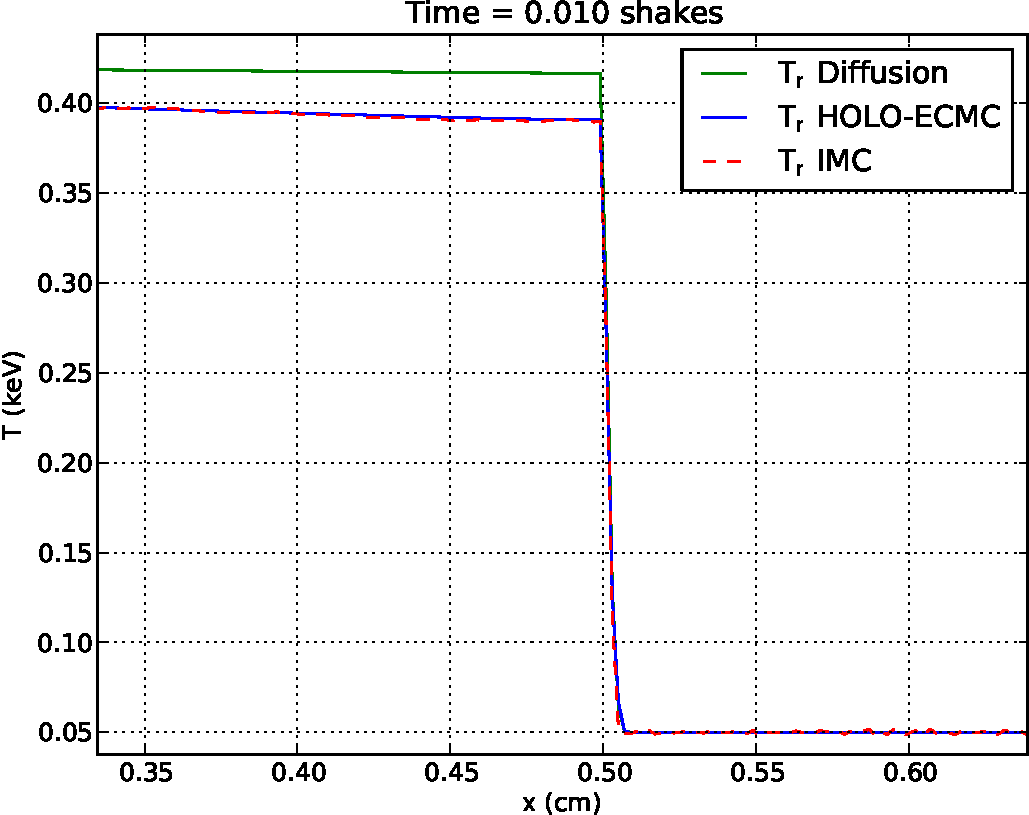
\includegraphics[width=0.59\textwidth]{twomat_holo_quick.pdf}
    \caption{Comparison of radiation temperatures for HOLO-ECMC, IMC, and diffusion for two material problem after 10 time steps. \label{twomat_quick}}
\end{figure}
    \begin{figure}
    \centering
    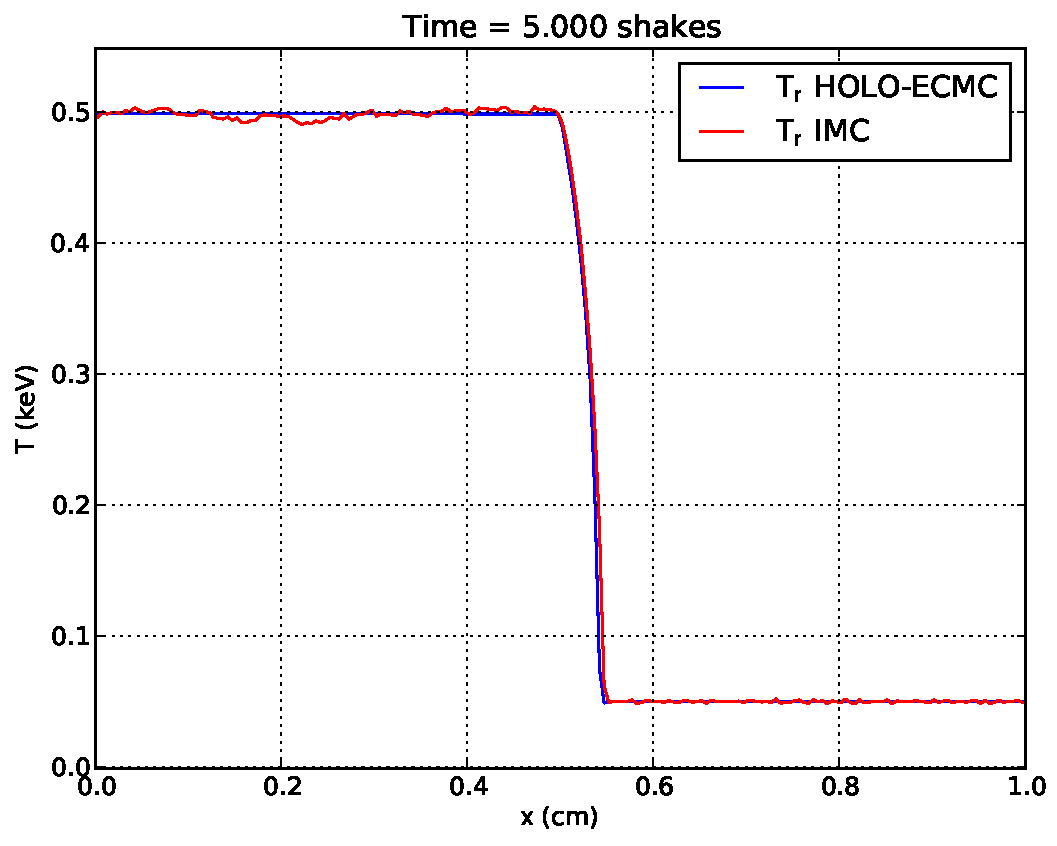
\includegraphics[width=0.59\textwidth]{twomat_full.pdf}
    \caption{Radiation temperature profiles for two material problem after 5 shakes.\label{twomat_full}}
    \end{figure}

\Subsection{Marshak Wave}

For this problem, initially the radiation and material energies are in equilibrium at 2.5E-05 keV.   An isotropic incident intensity of 0.150 keV
is applied at $x=0$ at $t=0$; the incident intensity on the right boundary is 2.5E-05 keV.  The material properties are $\rho = 1$ g cm$^-3$ and $c_v = 0.013784$ jks/keV-g. The absorption cross section varies as
\begin{equation}
\sigma(T) = \frac{0.001 \rho}{T^3},
\end{equation}
which introduces a strong non-linearity into the problem.   The simulation was ran for 5 shakes with a
time step size of 0.001 shakes. 

Fig.~\ref{marshak_holo_ld} compares the cell average radiation temperatures for the IMC and HOLO methods.  The radiation wave front is significantly farther ahead in the HOLO method.  Simluations with a refined mesh and time step did not remove this discrepancy, and the IMC solution did not move much.  This suggest that the fact that IMC lags opacities is not the cause of the difference.  There are a couple notable issues that could be the cause of the discrepancy.  Although the averages are positive, the LD representation of the intensity leads to engativites near the steep wave front.  The negativities lead to poor consistency terms.  Additionally, histories with large negative weights in the wave-front region enter the equilibrium cells to the right and cause poor statistics due to the thick cross section.  This leads to consistency terms that are unphysical ($\mom{\mu} \notin [ -1, 1]$) in cells near the wave front.  In these cells diffusion equivalent  parameters are used for the parameters that are bad.  The diffusion approximation near the wave front ultimately leads to a faster wave speed.  There are a couple ideas discussed in future work for correcting the bad statistics on the right side of the wave front.

Fig.~\ref{blading} plots the LD representation of the material and radiation energies (in this figure the negativities in the radiation are plotted as zero, but due exist at the wave front).  The steep, unphysical gradients in the material temperature distribution are a result of using cell-wise constant cross sections.  More accurate, spatially varying cross sections will be implemented in future work.  

To correct issues introduced into the LO solver by negativities in the radiation equation, the lumped-equivalent spatial discretization discussed previously was implemented for the LO solver.  The HO solver was left as LD in space in angle.  Thus, the LO discretization preserves the $L$ and $R$ moments of the HO solution, but does not use a consistent outflow.  Results with this alternative LO discretization are displayed in Fig.~\ref{lumped_marshak}.  The wave speeds are much closer, but there is still a noticeable discrepancy.   The first and easiest method for resolving this issue would be to implement a similar strictly positive discretization in the HO solver to ensure consistency.  This will likely resolve some of the issues with noise resulting in bad consistency terms.
    \begin{figure}
    \centering
    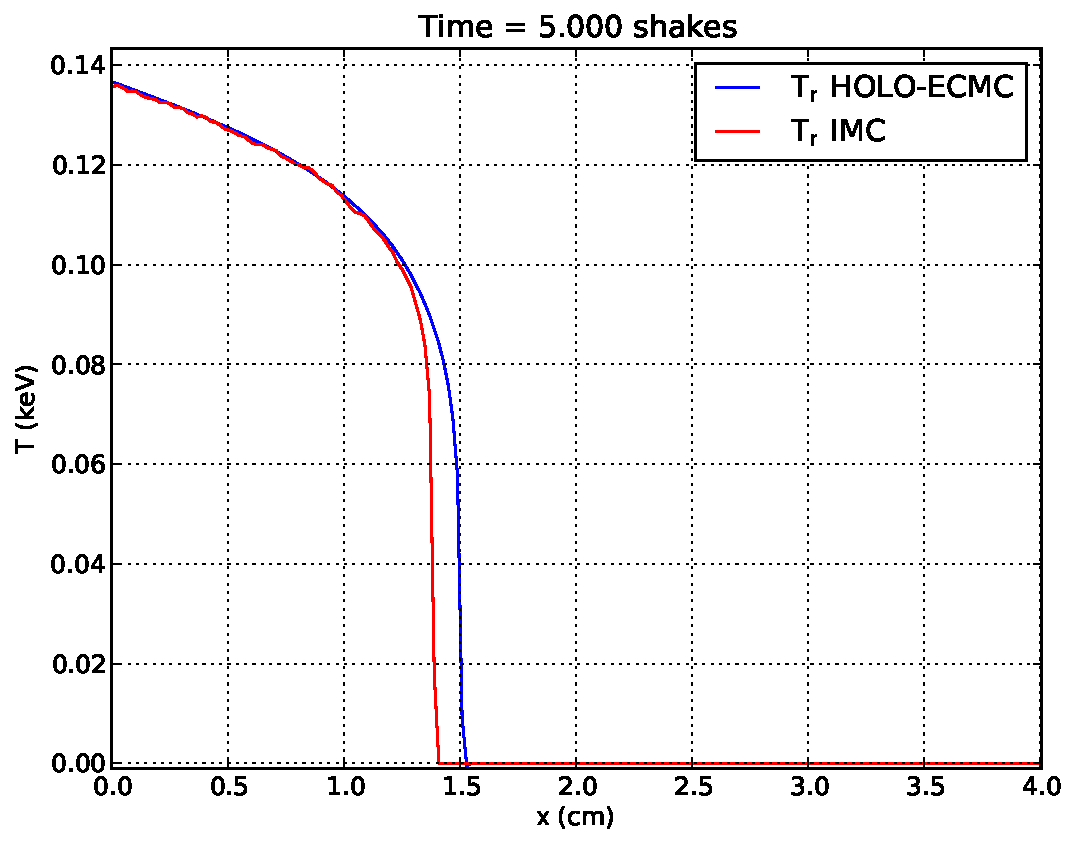
\includegraphics[width=0.59\textwidth]{marshak_holo_ld.pdf}
    \caption{\label{marshak_holo_ld} Comparsion of cell-averaged radiation temperatures for Marshak wave problem.}
    \end{figure}
    \begin{figure}
        \centering
    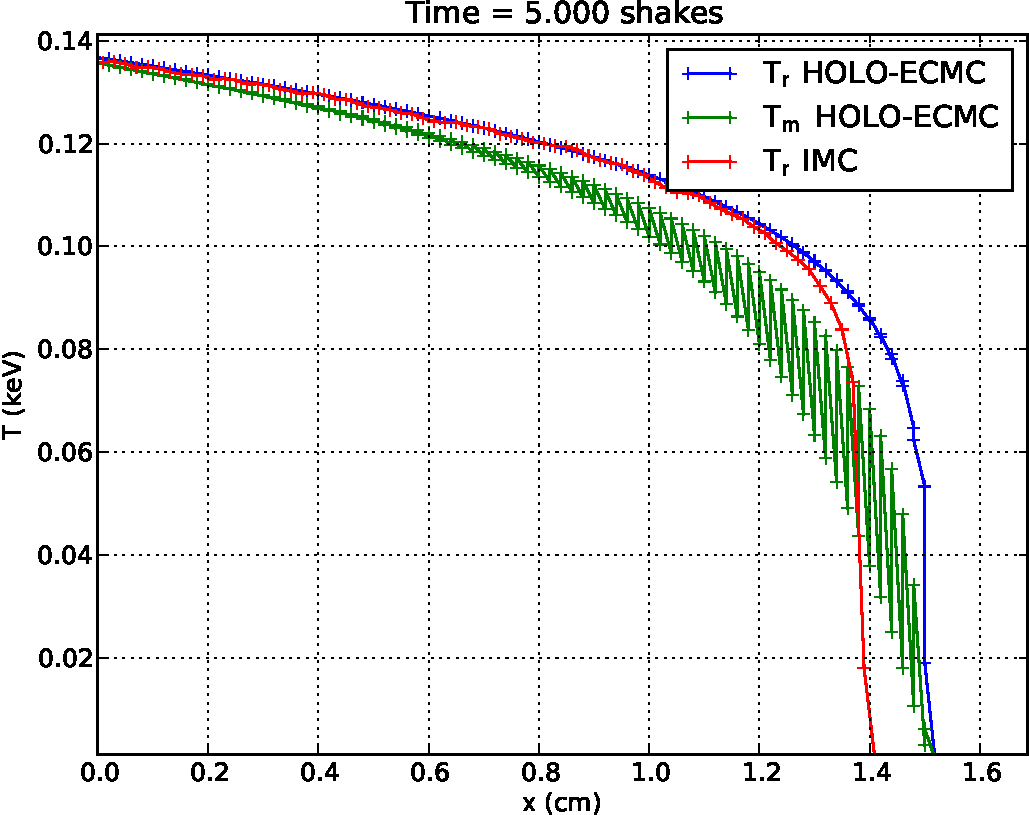
\includegraphics[width=0.59\textwidth]{blading.pdf}
        \caption{\label{blading} LD representation of material and radiation energy temperatures for HOLO, as compared to cell averages for IMC, for Marshak wave problem.}
    \end{figure}
    \begin{figure}
        \centering
    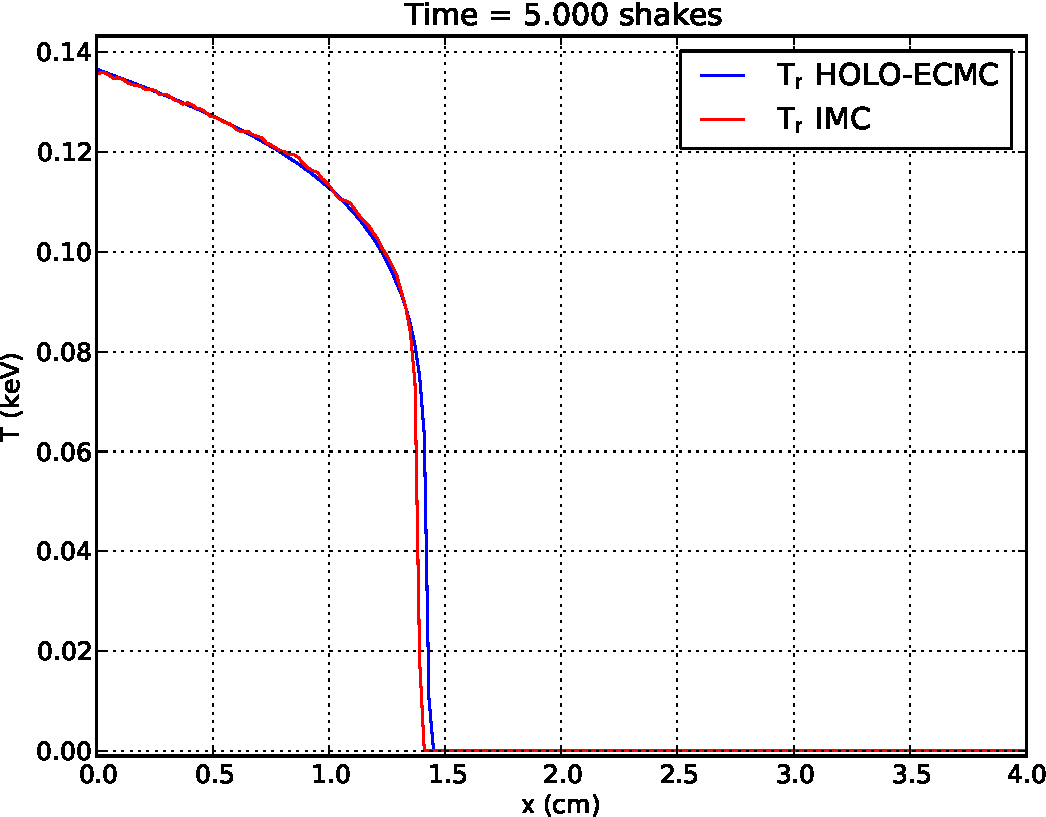
\includegraphics[width=0.59\textwidth]{marshak_holo_lumped.pdf}
        \caption{\label{lumped_marshak} Marshak wave problem with lumped-equivalentLD spatial representation for  LO
        solver.}
    \end{figure}

\Section{Conclusions}

We have been able to reproduce the IMC solutions for certain problems using a new HOLO method.  The primary difficulty is in the speed of wave fronts for the Marshak wave problem.  The LO solver resolves the non-linearities in the equations resulting in a fully implicit time discretization.  The ECMC approach, with initial guesses based on the previous radiation intensity, results in efficient reduction of statistical error and allows for particles to be distributed to largely varying regions of the problem.  Analytic transport benchmark results are
needed for a direct comparison of the accuracy between the HOLO and IMC methods.  However, most of
the transport benchmarks utilize reflective boundary conditions.
Reflective boundary conditions have been successfully implemented in the LO solver,
but have not yet been successfully implemented in the HO solver.  An explanation of the
difficulties with reflective boundary conditions is detailed in the Appendix.  Once
the reflective boundary conditions are correctly implemented, a comparison of the
accuracy of the two methods can be made.

Other future work will include continuous energy deposition tallies as a form of variance reduction.  Also, a strictly positive spatial discretization in the HO system will be implemented.  If this does not resolve issues with statistical noise, a form of cell-wise error filtering will be implemented.  With the exception of the first batch, it is not expected that the relative error in a cell should be less than 1.  If this is the case, then it is likely due to a bad MC estimate.  These cases could be rejected and the previous estimate of the intensity in that cell used for the next calculation, or a damped version of the change could be used.    Long term work will include adding the ability to handle opacities that vary as lLD with temperature in space.  A multigroup formulation will be explored, before extending to multiple spatial dimensions.

\bibliography{references}
\bibliographystyle{unsrt}    
\clearpage

\appendix

\Section{SECOND OR SUBSEQUENT MAJOR HEADING} 
\label{sec:first}

This is Section~\ref{sec:first}. It is followed by a Subsection, that is, 
\ref{sec:second}. For this class file you must use the 
\texttt{$\backslash$Section\{\}} to denote sections (note the capital ``S'').  
The style for subsection titles and all text in this template is defined in 
the {\it mc2013.cls} file.  Make sure to avoid widow/orphan lines.


\Subsection{Subsection Title: First Character of Each Non-trivial Word is 
Uppercase} 
\label{sec:second}

Double-space before and after secondary titles is automatic.  Figures and 
tables should appear as close as possible to where they are first
cited, e.g., Fig. \ref{fig:amdahl}, in the text.  Figures are numbered in 
Arabic numerals, with the caption centered below the figure, in 
{\bf boldface}.
  
Triple-space before the figure, and after the figure caption.

%
\vspace{16pt}
\begin{figure}[!htb]
\begin{spacing}{1.0}
\centering
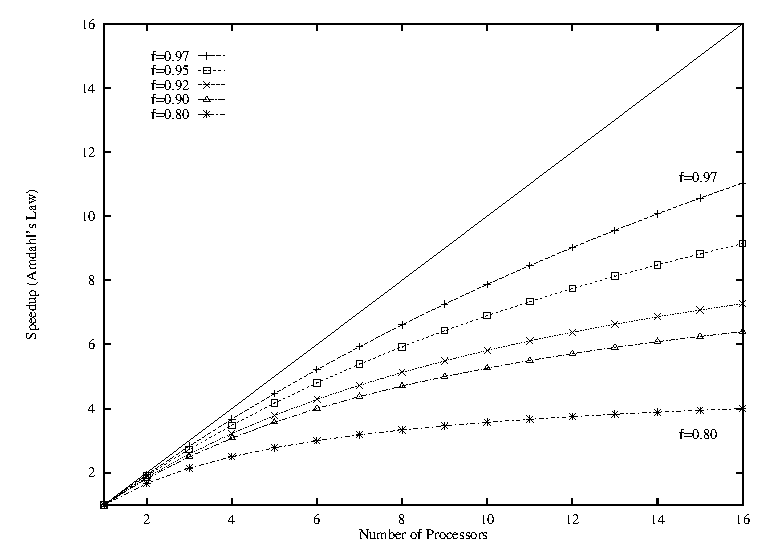
\includegraphics[scale=0.60]{./figure.eps}
\caption{\bf Speedup vs Number of Processors for Varying Parallelizable 
Fractions in Order to See a Multiple Line Caption} 
\label{fig:amdahl}
\end{spacing}
\end{figure}
\vspace{16pt}
%

When importing figures or any graphical image please verify two things:
\begin{itemize}
\item Any number, text or symbol is in Times font and is not smaller than 
    10-point after reduction to the actual window in your paper
\item That is can be translated into PDF
\end{itemize}


Equations, such as Eq. (\ref{sample_equation}), should be centered and 
sequentially numbered to the flush right of the formula.
\begin{equation}
\label{sample_equation}
Speedup\ =\ {1 \over{{f \over {p}} + (1-f)}}
\end{equation}
The continuation of a paragraph after an equation should not be indented.  
All paragraphs, as well as section or subsection headings, are separated by 
just one single empty line.


\Subsubsection{Sub-section level and lower: only first character uppercase}

See Table \ref{table:example} for a sample table.  The tabls package is
recommended for improved row and column spacing.  Notice the caption appears 
above the table by setting the \texttt{$\backslash$caption} command immediately 
after the \texttt{$\backslash$begin\{table\}}. Tables are numbered in Roman 
numerals, with the caption centered above the table, in {\bf boldface}.  
Triple-space before and after the table.

\vspace{16pt}
\begin{table}[!htb]
\centering
\caption{\bf Parallel Performance for the Sample Problem}
\label{table:example} 
\vspace{14pt}
\begin{tabular}{||r||c|c|c||} \hline \hline
 \multicolumn{1}{||c||}{Number of} &
 \multicolumn{1}{c|}{Wall-Clock} &
 \multicolumn{1}{c|}{Speedup} &
 \multicolumn{1}{c||}{Efficiency} \\
 \multicolumn{1}{||c||}{Processors} &
 \multicolumn{1}{c|}{Time$^{a}$ (min)} &
 \multicolumn{1}{c|}{(T$_{s}$/T$_{p}$)} &
 \multicolumn{1}{c||}{(\%)} \\ \hline\hline
\ 1 &  100.0 & \ ---    & ---  \\ \hline
\ 2 &   52.6 & \ 1.9    & 95.0 \\ \hline \hline
\end{tabular}
\end{table}
\vspace{16pt}


\Section{CONCLUSIONS}

Present your summary and conclusions here.


\section*{ACKNOWLEDGEMENTS}

This research was performed, in part, using funding received from the DOE Office of Nuclear
Energy's Nuclear Energy University Programs.


%\Section*{REFERENCES}
\setlength{\baselineskip}{12pt}
\begin{thebibliography}{300}
\bibitem{journal} B. Author(s), ``Title,'' {\it Journal Name in Italic}, 
          {\bf Volume in Bold}, pp. 34-89 (19xx).
\bibitem{willert} J. Willert, C.T. Kelly, D.A. Knoll, and H. Park,
         ``A Hybrid Approach to the Neutron Transport k-Eigenvalue Problem using
         NDA-based Algorithms,'' {\it M\&C}, Sun Valley, ID, May 5-9 (2013).
\bibitem{park} H. Park, J.D. Densmore, A.B. Wollaber, D.A. Knoll and  R.M. Ramenzahn,
                ``Monte Carlo Solution Methods in a Moment-Based Scale-Bridging
                Algoirthm for Thermal Radiative Transfer Problems: Comparison with
                Fleck and Cummings,'' {\it M\&C}, Sun Valley, ID, May 5-9 (2013).
\bibitem{book} E. F. Author, {\it Book Title in Italic}, Publisher, City \&
          Country (19xx). 
\bibitem{website} ``Spallation Neutron Source: The next-generation 
          neutron-scattering facility in the United States,'' 
          http://www.sns.gov/documentation/sns\_brochure.pdf (2002).
\end{thebibliography}

\end{document}


